
\documentclass[12pt]{article}
\usepackage{graphicx}
\usepackage{caption}
\usepackage{natbib}
\usepackage{authblk}
\usepackage[utf8]{inputenc}
\usepackage{setspace}
\usepackage{rotating}
\usepackage[british]{datetime2}
\usepackage{hyperref}

\renewcommand{\harvardurl}{\textbf{URL:} \url}

\renewcommand\Affilfont{\itshape\small}

\title{Dynamics of Armed Conflict Essay}
\author[1]{Marius Swane Wishman}
\affil[1]{Department of Sociology and Political Science, NTNU}

\date{\today}

\providecommand{\keywords}[1]
{
	\small	
	\textbf{\textit{Keywords---}} #1
}

\begin{document}

\maketitle

\begin{abstract}

\end{abstract}

\keywords{}

\pagebreak

%tableofcontents
%\pagebreak

\onehalfspacing

\section{Introduction}

Growing literature on pre-colonial states and civil conflict.

\section{Theory}

\subsection{Conflict reducing}

\subsubsection{Internal monopoly of violence}

The \citet{Tilly1990} argument, 
%TODO: infuse more Tilly into the mix, other relevant authors? 
States as stationary bandits gradually remove internal
competitors. Over time this reduces the number of actors within the borders of a
state that are able to wield organized forms of violence, and the remaining
ones' ability to do so. In the case of pre-colonial states, they are now either
once again `the' state (for example Morocco or Ashanti/Ghana), have been
incorporated into a larger state as part of its apparatus, or had its
institutions destroyed by some larger state (colonial or indigenous)
consolidating its role as the sole stationary bandit within its borders. In
other words within the former borders of a pre-colonial state there should be a
reduced number of potential wielders of organized violence (ceteris paribus)
depending on the pre-colonial states centralization/consolidation, itself a
product of time, reforms/political organization/idiosyncrasies and the proximity
to its capital. If the pre-colonial state was incorporated only partially into
the modern state, it could still pose a threat to the central state through
desertion (more on this later). If the pre-colonial state was destroyed, for
example by colonizers, without new state (colonial or post-colonial) entering
the resulting power vacuum other actors would do so, and become new stationary
bandits rivalling the state. How does this compare to other areas not formally
part of a pre-colonial state? These areas could inhabit roving bandits
\citep{Scott2009} or other actors already having filled an equivalent vacuum of
power. In other words, in this scenario pre-colonial state areas should be no
worse than other areas in terms of violence. Any resulting conflict running
through this mechanism should occur shortly after decolonization.

\subsubsection{Better Angles}

\citet{Pinker2012} builds an argument from cognitive science affective and
cognitive neuroscience, social and evolutionary  psychology, that humans are
capable of producing a lot of violence, but also show a lot of restraint and
compassion. It  all depends on the structures surrounding us, and how we are
socialised. He seeks to explain the extraordinary levels of
violence\footnote{\citet{Pinker2012} examines a number of forms of violence,
	both organized, unorganized, interpersonal, state based, international
and intra-national.} evident in the historical and archaeological record, and
its decline to modern levels.  Of relevance here, \citet{Pinker2012} identifies
five `trends' and five `historical forces' (as well as nine aspects of our
psychology, five promoting violence and four inhibiting it), that he uses
explain the observed decline in violence. The two first trends are the invention
of agriculture, the first cities and \textit{governments}. Early states
`pacified' their population following the logic of Hobbes Leviathan.  Leading to
an estimated fivefold reduction in likelihood of dying a violent death. Second,
the consolidation of large \textit{kingdoms with centralized authority} and an
infrastructure of commerce engaged their citizens in a `civilizing process',
whereby people were able to think and plan more long term.  This promoted acting
more rational (as \textit{homo economicus}) and inhibit impulsiveness to engage
in ever more positive sum games, leading to further reductions in violence at
individual, regional and country level. Again, the state (and increasing
commerce in this case) are the exogenous factor that sets the virtuous cycle in
motion. In addition, as polities become fewer and larger there is a reduction in
the number of actors that can engage in large scale/organized violence, leading
to fewer albeit bloodier conflicts. Nevertheless, the over all negative trend of
violent death continues. Partly as a result in the reduction in conflicts
outweigh their increased lethality, but partly also because of the reduction of
violence within polities. Citing \citet{richardson1960statistics}
\citet{Pinker2012} states that when area is held constant, there are far fewer
civil wars within borders than than there are interstate wars crossing them.
\citet{Pinker2012} also reiterates Tilly and Hobbes logic that ``As small
baronies and duchies coalesced into larger kingdoms, the centralized
authorities prevented them from warring with each other for the same reason that
they prevented individual citizens from warring with each other (and that
farmers prevent their livestock from killing each other): as far as an overlord
is concerned, private quarrels within his domain are a dead loss."

Of the `historical forces', the first is the `\textit{Leviathan}'; ``a state and
judiciary with a monopoly on the legitimate use of force, can defuse the
temptation of exploitative attack, inhibit the impulse for revenge and
circumvent the self-serving biases that make all parties believe they are on the
side of the angels." \citep[xxvi]{Pinker2012}. \citet{Pinker2012} goes as far as
concluding that the Leviathan ``may be the most consistent violence-reducer that
we have encountered in this book." \citep[680]{Pinker2012}. The contribution of
\citet{Pinker2012} is the synthesis of political and social science theories
with psychology. Critically, he shows that the self-control and aggression
reducing effects of the Leviathan can become habits so that citizens refrain
from violence ``Even when Leviathan's back is turned." \citep[681]{Pinker2012}. In
\citet{Pinker2012}'s eyes then, states, and the evolution of states have played
a big role in the historic decline of violence through shaping the environment
of its citizens to be more inducive to peace. If Pinker is right in thinking
that the formation and growth/expansion of states puts societies on a track
toward more peaceful societies, then areas with \textit{longer} and
\textit{deeper} histories of statehood should exhibit the effects of this, even
after 150-200 years. Working through the mechanisms of the interplay between
Leviathan and `gentle commerce', internalising or habitualising and perhaps
institutional inheritance (governance evolves so that areas that had some
governance in the past have better governance today).

\subsubsection{Mechanisms}

Leviathan x gentile commerce. \textit{proxied} by higher levels of development
in areas of higher state presence. Predicts lower levels of violence in areas of
higher state presence, working \textit{through} development.

If past state presence is positively correlated with post-independence state
presence, then both the leviathan/pacifying and civilising mechanisms predict
less violence in high state presence areas.

Habitation/internalisation predicts lower levels of violence in higher state
presence areas \textit{contingent} on \textit{continuation} of state presence,
as this is quickly `unlearned'.

% Difficult to separate the effects of these mechanisms from others.

\subsubsection{Credible commitments}

\citet{Wig2016} argues that ethnic groups with ties to pre-colonial statehood
are more likely to have inherited institutions that allow the ethnic group to
punish defections and hold their leaders accountable.  In this way, ethnic
groups with ties to pre-colonial statehood are better able to make credible
commitments, than 'non-state' ethnic groups.  Credible commitments help such
groups both prevent conflict from occurring in the first place, but also make
them better able to end conflicts when then they have broken out.  Empirically
\citet{Wig2016} finds that groups with histories of statehood do indeed
experience less dyadic conflict with their government.
\citet{Depetris-Chauvin2016} makes a similar argument and finds that regions
with exposure to pre-colonial statehood are more peaceful, \textit{ceteris
paribus}.

\subsubsection{Alternatives to Violence}

Inherited pre-colonial institutions could also provide conflict resolution
mechanisms (or institutions) that allow local conflicts to deescalate or be
resolved before escalating to violence. ** Examples **

%\subsubsection{Economic advantage?}

\subsection{Conflict inducing}

\subsection{Symbols of past sovereignty}

Symbols to rally around as well as a foundation for ethnic claims making
following the international adoption of the policy of self determination of
peoples.

\subsection{Networks useful for insurgency}

Pre-colonial states can leave behind formal and informal social networks that
lower the cost of insurgent collective action \citep{Wig2016, Wood2000}. The
most visible examples of this are cases in which kingdoms were ruled indirectly
and remained intact into the modern era. Buganda, Lunda-Yeke, Aussa examples.

\subsubsection{Central State Weakness/Collapse}

When modern states `collapse' or in another sense achieve `failed state' status,
it creates a (series of) power vacuums and room/need for other actors to fill
the various roles usually filled by the state. At the regional level one can
imagine a handful of actors capable of filling this vacuum (of power and
service provision), one of which is pre-colonial state. Other candidates could
be active rebel groups, religious organizations and ethnic groups (not tied to
pre-colonial states). I would argue that pre-colonial states and active rebel
groups have distinct advantages above the others. Prime mover advantage and
capacity to monopolise violence on part of rebel groups, and legitimacy and
organizational benefits on the part of pre-colonial states.

The dynamics of this lie in how state collapse unfolds and `evolves'. Although I
am not sure if I will be able to test or properly examine this process I will
nevertheless sketch out how I imagine it (typically) unfolds.

Democratic collapse, succession/reform crises, state predation and/or civil war
are usually on the path toward state failure\citep{Goldstone_2008}. Once a state
has failed, lost its legitimacy and effectiveness \citep{Goldstone_2008}, other
actors will attempt to fill the void. This happens at all levels of government I
imagine, but most visibly at the country (repeated coups, attempts to overthrow
the government) and regional level (various forms of regional self governance).
I will focus on pre-colonial states reemerging as a basis of regional self
governance  (RSG) and the dynamics of it. If or when a pre-colonial state,
through either ethnic group, formal institutions or less formal networks, begins
to engage in RSG it sets out on a path that will at some point clash with the
interests of the central government. Because of its position as a pre-colonial
\textit{state} it is inevitably a challenge to the integrity of the state as a
whole. This creates a potential for further conflict, along new lines, in often
war torn countries. 

A different aspect of pre-colonial states engaging in RSG is that they can
create pockets of relatively functioning government within otherwise failed
states. I believe this can at least be tentatively explored on few case-by-case
basis using the data I have available. Do areas of high state presence (see data
section) outside the capital, experience a drop in combat events after engaging
in RSG. 

The example I primarily had in mind is  Puntland in Somaila, which corresponds
to the pre-colonial state of the Majarteen sultanate, has engaged in RSG as an
autonomous state within Somailas federal system. In terms of both peace and
prosperity the region has fared better than the rest of Somalia. Unlike
Somaliland the state is not seeking full independence. However, they do have
their own military forcer and tensions could rise if the central government were
to attempt further integration.

Other potential cases in Africa (see data) include Chad, Nigeria, DRC,
Sudan/Darfur and Lebanon.

Consider the illustrative case of the Russian federal state of Tatarstan. The
Tatar Khanate of Kazan was conquered by Ivan the Terrible in 1552 and
incorporated into the Russian empire as Kazan province by Peter the Great in
1708 \citep{Sharifzhanov_2007}. Despite Russification policies until the reign
of Cathrine II the Great (1762-96), when the Russian Empire collapsed following
the February revolution of 1917 Tatar nationalist seized the moment and declared
the creation Idel-Ural state \citep{Devlet_1993}. The nascent state laid claim
to boundaries closely resembling those of the old Khanate \citep{Hartley2020},
but the Bolsheviks and the Red Army were able to thwart the secession after a
month \citep{Hartley2020}. While the Tatars of Kazan no doubt were able to
retained their dreams of independence in large part to the ethnic and religious
differences between themselves and their rulers, it is striking that the
proposed borders follow those of the old Khanate and not of settlement patterns
of the Tatar ethnic group who were spread over a larger territory as part of the
Russification policy of the Tsars. Part of the movements goals was also the also
to allow Tatars émigré populations to return to their homeland
\citep{Devlet_1993}. When in turn the Soviet Union began to open up and collapse
in 1990-1991, the space once again opened up for the Tatars to reassert their
sovereignty. Following the example of Moscow and Russia the Tatar Autonomous
Soviet Socialist Republic declared itself a sovereign republic within the USSR,
which it attained in a declaration adopted by the Supreme Soviet. Thus on 12
June 1991 Russia acquired two presidents, Boris Yeltsin and Mintimir Sheymiev
\citep{Sharifzhanov_2007}. A referendum was set for 21 March 1992 on the
question of Tatarstan's independence. Authorities in Moscow tried to prevent
the referendum through the Constitutional Court of Russia and televised appeal
by Yeltsin to boycott the referendum, warning that an affirmative response
``would possibly lead to bloodshed." \citep{Sharifzhanov_2007}.  Nevertheless,
the referendum went ahead in the presence of international observers and boasted
a turnout 82 percent of which 61.4 percent voted for independence
\citep{Devlet_1993}. Following the referendum a new constitution was drafted
confirming Tatarstan's sovereignty. ``The Republic of Tatarstan shall be a
sovereign state, a subject of international law, associated to the Russian
Federation - Russia - on the basis of the Treaty on Mutual Delegation of Powers
and Subjects under Jurisdiction." \citet{Sharifzhanov_2007}. Unlike Chechen
leaders the Tatar leaders did not threaten use violent resistance to secede from
Russia, and through negotiations with the Yeltsin government they were able to
carve out a unique position of autonomy within the Russian Federation in 1994.
The different positions on the use of violence between the Chechens and Tatars
I believe is due to the feasibility of armed resistance to even a greatly
weakened Russian state based on geographic conditions. Chechnya is on the very
edge of the Russian periphery and is a mountainous country. Tatarstan on the
other hand lies relatively close to Moscow, and its steppe terrain lends an
advantage to modern national armies. In the words of the Chairman of the
Tatarstan parliament: ``We take a completely \textit{realistic} view of the
state of affairs: full independence is too abstract and unnecessary a concept
whereas Tatarstan and Russia are linked by inseparable bonds."
\citep{Sharifzhanov_2007}(emphasis added). At the same time parallels were still
drawn all the way back to the Kazan Khanate. During a speech at the first World
Congress of Tatars the Tatarstan president Mintimir Sheymiev declared that:

\textit{The history of the Tatars nation is very difficult and tragic. The
Tatars lost their Bulgar state, but found a respectable place for themselves
within the Golden Horde. After its collapse they created the khanates of Kazan
[...] the restoration of statehood was an idea ever present in Tatar history.}
(cited in \citet{mustafin1995pervyi}, 113).

Hx: Areas of high SP, far from capital will experience more conflict following
situations of state collapse.

\subsubsection{Political Inequality}

In countries where an ethnic group has a history of statecraft, said group is
likely to be have an over sized share of power in government. This can come
about through indirect colonial rule, which preferred to leave existing power
structures intact, or by seizure from less politically experienced groups
following independence \citep{Paine2019}. \citet{Paine2019} argues that such
state groups are likely to either exclude other groups from power, leaving them
with few options outside violence to achieve political representation. Or, in
the cases where state groups are are excluded themselves, they have the means to
organize and solve the necessary collective action problems and will reclaim
their dominating position by force \citep{Paine2019}. In case of fighting then,
it would happen in the area of the state group only in the cases where that
group was excluded from power. However, using our more fine grained data it is
apparent that this is far more common than \citet{Paine2019} supposes. *** High
SP far from the capital, could proxy (at least) this mechanism. *** The other
case predicts fighting in areas of excluded groups. *** I could tease this out
using the geo-epr data for areas of excluded groups with low levels of SP, or
simply predict high levels of conflict in areas of high population, but low SP
in countries with high SP in the capital.*** In \citet{Paine2019}'s data there
are no instances of multiple state groups in one country, and so he does not
account for this in his theory. However, in our more exhaustive data this occurs
in several countries *** find exact number ***. Following \citet{Paine2019}'s
logic however, it would be expected that only one of the groups were handed (or
grabbed) the keys to the kingdom following independence, and that other state
group(s) would be relatively more likely to challenge any attempts at exclusion.
As this is a continuation of \citet{Paine2019}'s original mechanism, this would
also be best proxied by high levels of state presence far from the capital.

\subsubsection{Resistance to western influence}

That one article that argues that where European colonizers met
organized/powerful states (often Muslim), they more often either took longer to
colonise them or not at all, if/when they did they were integrated more
indirectly. This left these areas more isolated from western influences,
particularly that of protestant missionaries. If so, areas of higher states
presence should have been exposed to less western influences such as humanism,
`the escalator of reason' \citep{Pinker2012} and democracy.

Hx1: High levels of SP, far from the capital predicts higher levels of violence. 

Hx2: High levels of SP, far from the capital in countries with high levels of SP
in the capital predicts higher levels of violence. 

Hxm: Areas of higher levels of SP are less likely to be protestant, and/or
express support for humanist ideas (afrobarometer?). \footnote{`Humanist ideas'
as opposed to support for democracy because everyone supports democracy if you
ask them point blank, but everyone's definition of democracy does not conform to
a VDEM-sanctioned definition.}

\subsubsection{Multiple pre-colonial states}

Bargaining problems and multiplies any other effect.

Hx: High levels of SP, far from the capital interacted with the number of
pre-colonial states in the country predicts higher levels of violence.

\section{The Geo-ISD}

The main independent variable is a measure of what I call `state presence' per
PRIO grid cell. It is a measure of the aggregate presence of independent
pre-colonial states in the period 1800-1914. The data comes from the Geo-ISD
project where Charles Butcher (NTNU), myself and our excellent research
assistant Eirin Haugseth geocoded African states from the International Systems
Data (hereafter ISD) \citep{Griffiths2013}

To get the locations of different pre-colonial states we used a combination of
maps from the time period and maps found in historical atlases compiled by
modern historians that were covered by the ISD. The historically contemporary
maps were collected from the David Rumsey project at davidrumsey.com. We then
georeferenced the maps and traced polygons for the states included in both the
map and the ISD. Similarly the historical atlases were scanned, georeferenced
and relevant state entities were traced.

In the end we were left with over 3400 polygons covering the period 1800 to 1914
for continental Africa and Madagascar. For some pre-colonial states in the ISD
there were no maps for any years, some are covered only for some of the years
they are in the ISD, but a substantial number of them are covered by multiple
maps for many years. When maps disagreed on where the various borders were in a
given year, we take it as an indication of the ambiguity of where a given state
had \emph{de facto} or \emph{de jure} control in that year. In the areas where
all the maps agree we could be quite sure that the given state entity had real
presence.  While in areas where only one map indicated that the state was
presence, this could either be wrong, an indication of \emph{de jure} as opposed
to \emph{de facto} presence or some other form of limited presence. The coding
process of looking at hundred of maps strengthened this initial intuition, and
the resulting figures of state presence drawn from the complete data lends it
further credence. On aggregate most maps should agree on the core areas of a
state while the further away from the core fewer maps would consider the area
part of the state. We believe this approximates the real ambiguities surrounding
where states governed and where they did not, resulting in a measure of state
presence in a given area. Figure \ref{overlay} is an overlay of all the maps of
Libya, Tunisia and Egypt. It demonstrates how the authority of these states
faded into the desert, partially overlap at the borders, and in the Libyan case,
its tenuous hold on the Fezzan region. 

\begin{figure}[!htb]
	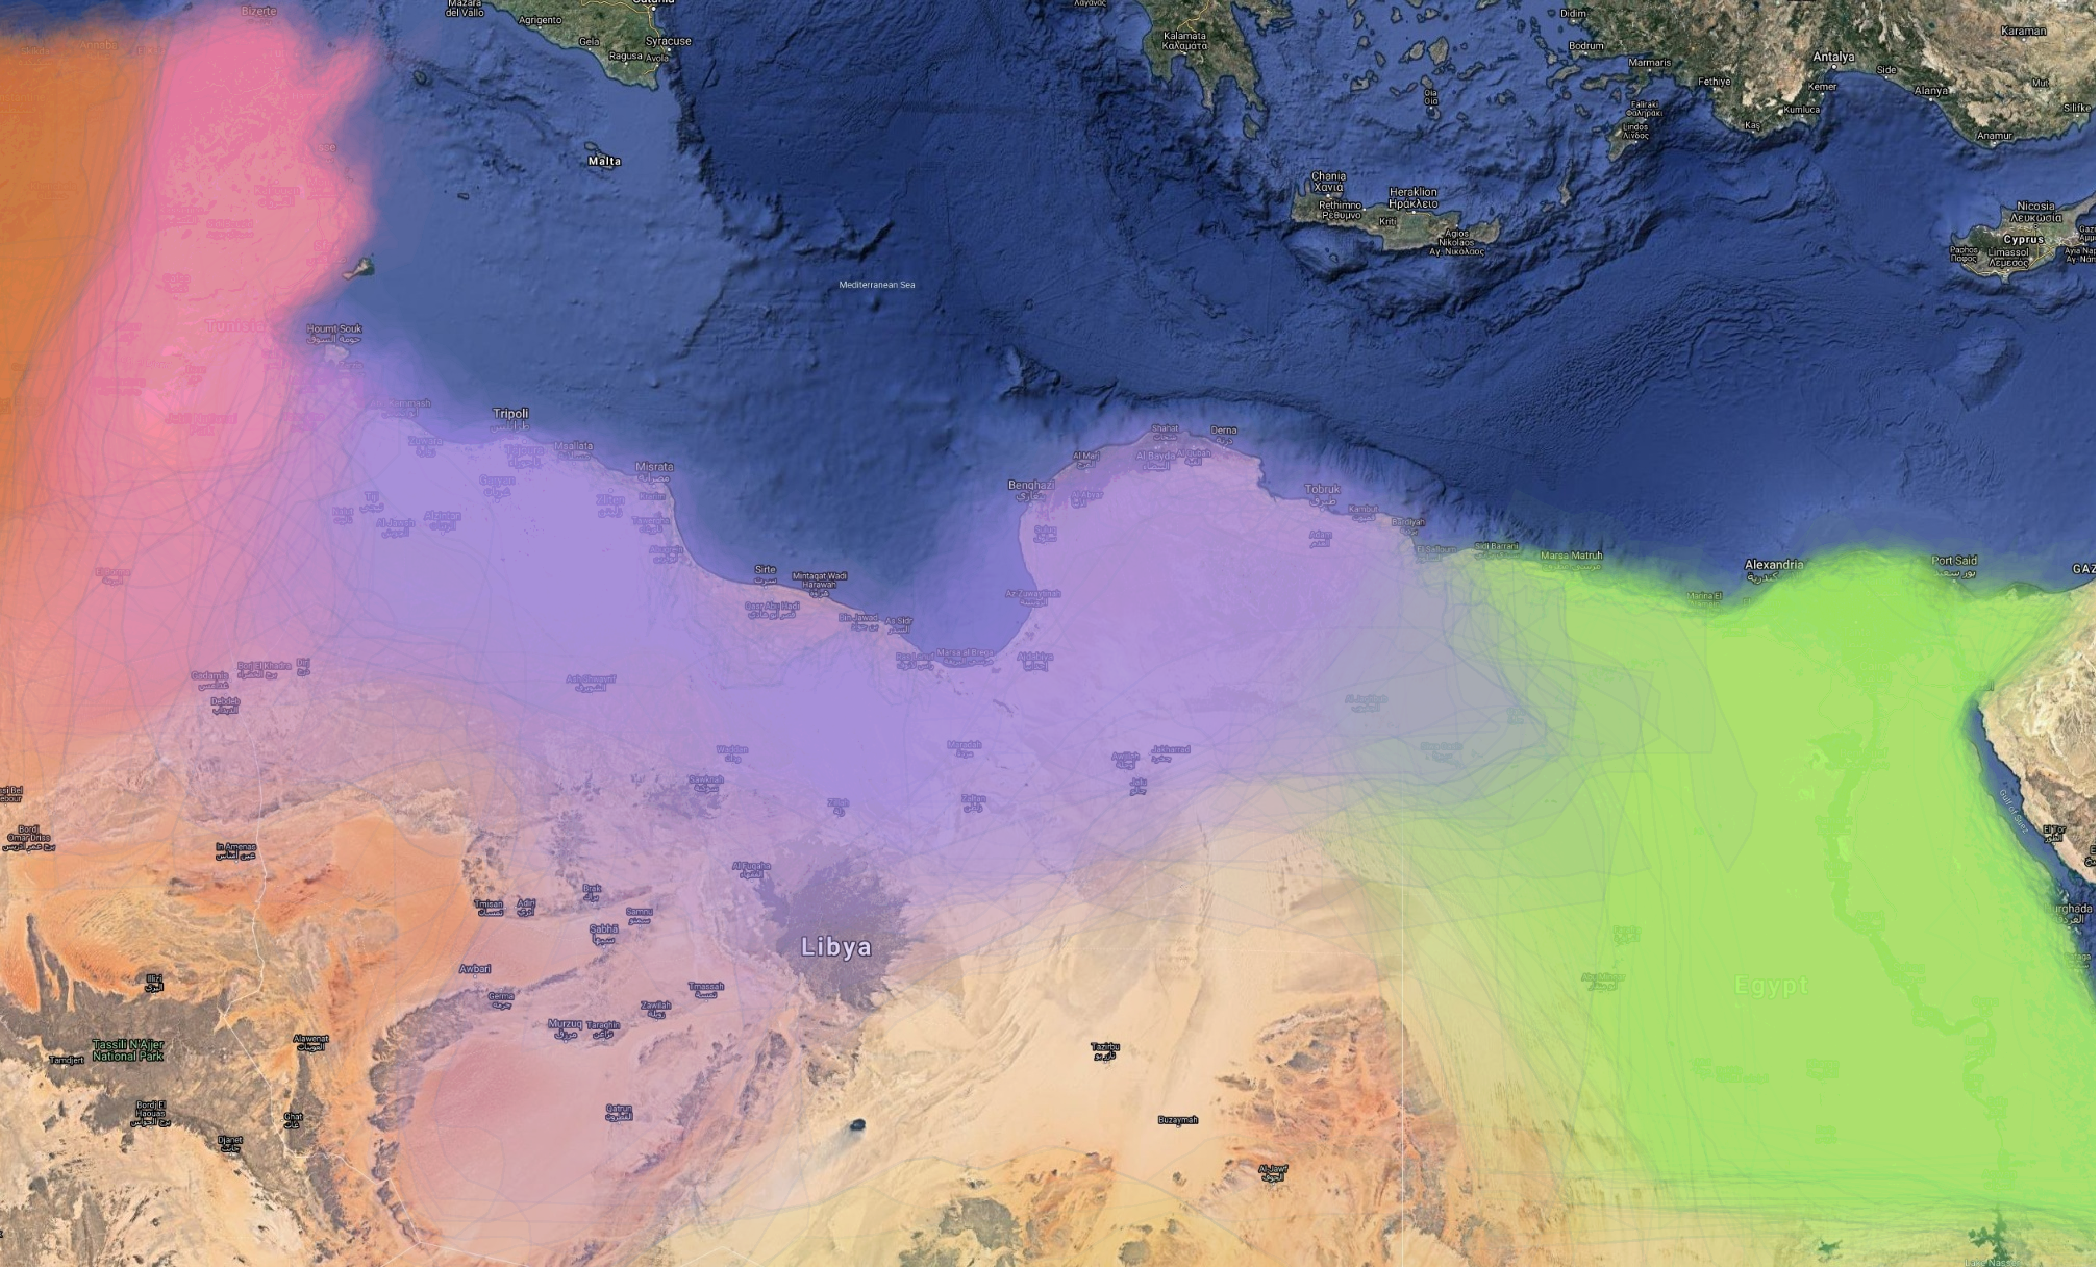
\includegraphics[width=\textwidth,keepaspectratio]{../TUNLIBEGY.pdf}
	\caption{Overlay of all maps of Tunisia, Libya and Egypt}
	\label{overlay}
\end{figure}

The data from this project can be aggregated and used in many ways and to
produce many variables. All of these indicators are aggregated over all years
for individual PRIO-GRID cells in Africa. The primary indicator used in this
essay is a measure of the presence of one state over time. It is measured by the
number of maps that indicate that a state was present there, counting only those
of the state most often present in that cell. Figure \ref{Sp} shows the log
transformation (to lessen the visual impact of large variations in the number of
maps for different states) of this measure for all African PRIO grid cells.

\begin{figure}[htpb]
	\centering
	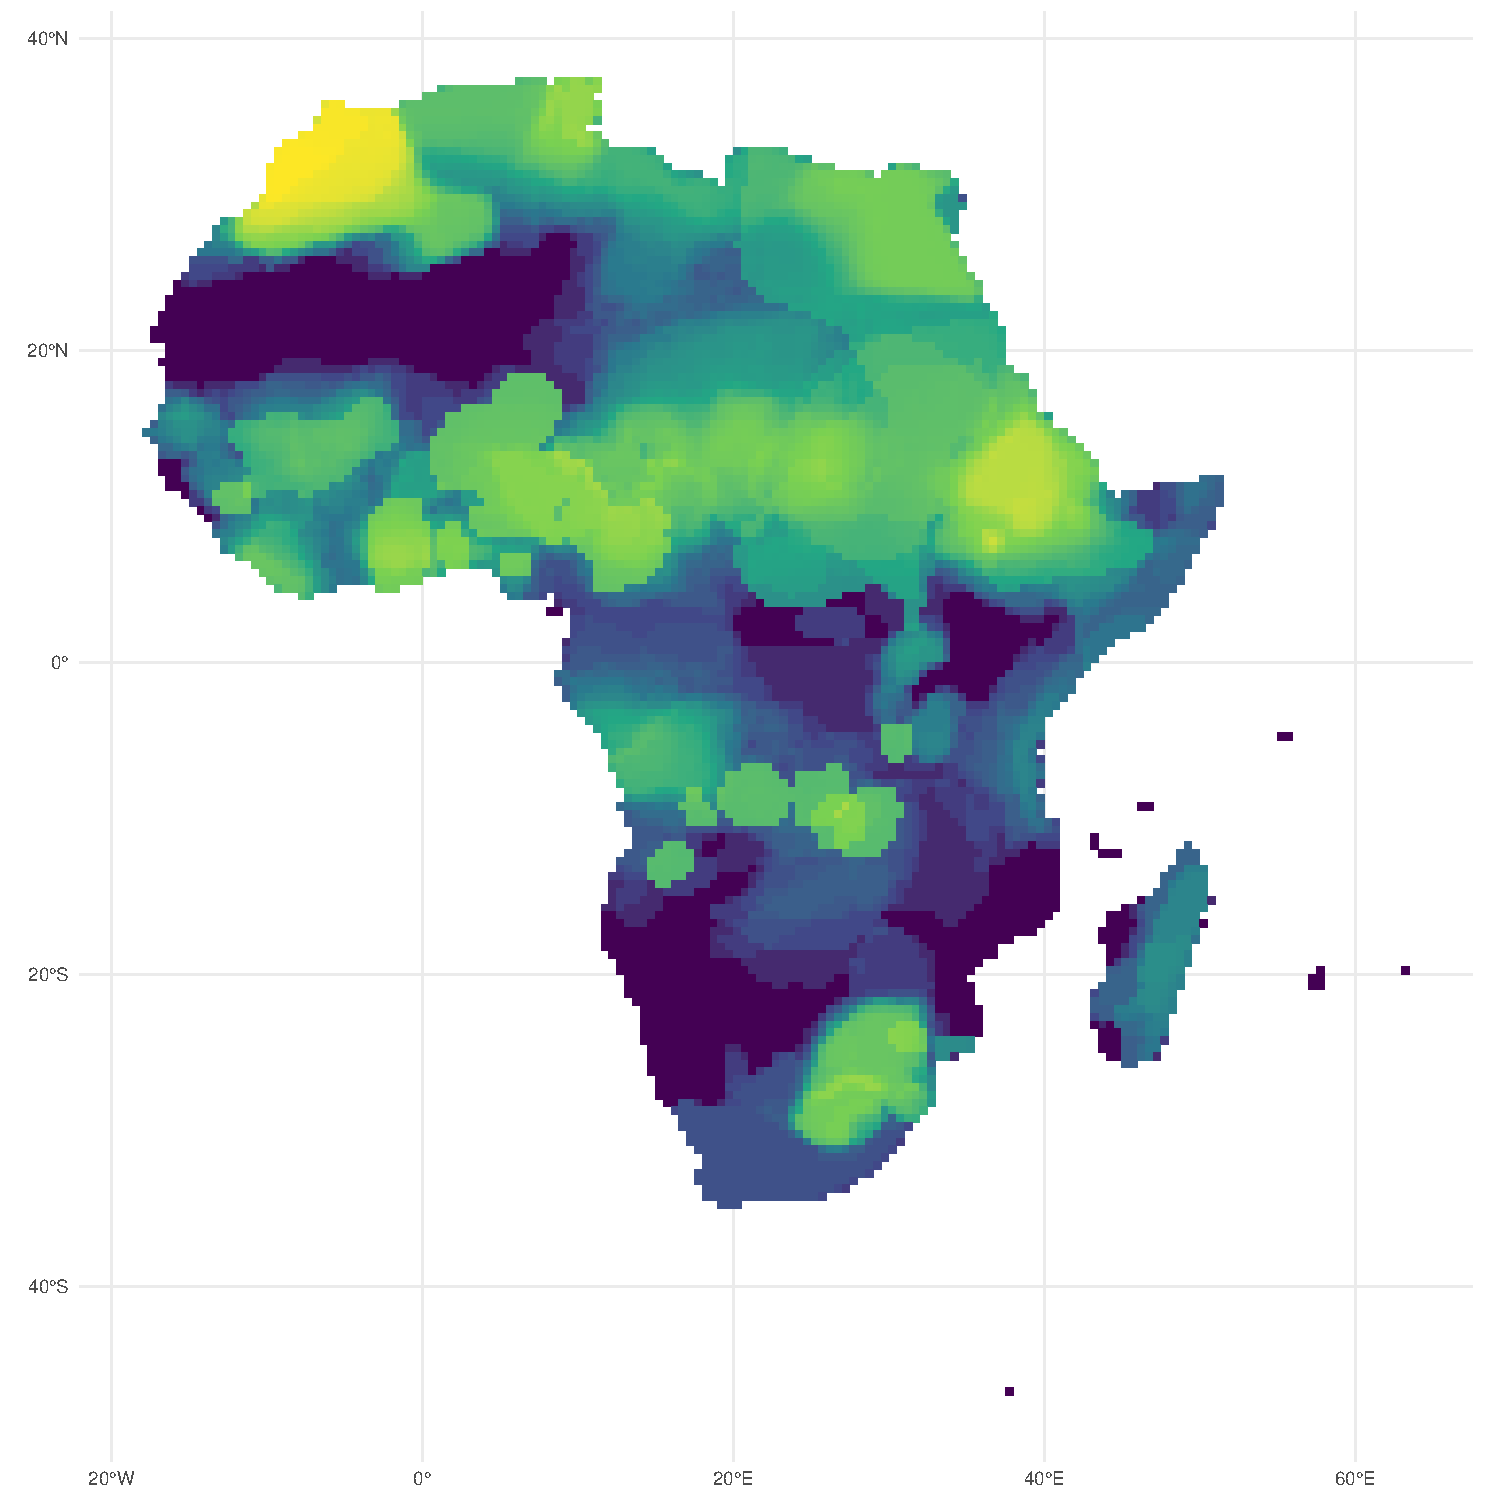
\includegraphics[width=0.8\linewidth]{../Rplot_ln_sp_int.pdf}
	\caption{State presence, log transformed}
	\label{Sp}
\end{figure}

\section{Research design}

\subsection{Dependent variable}

Unit of analysis is PRIO grid cell 

Fatalities - square root transformed and logged

State based conflict events - square root transformed and logged

\subsection{Independent variable}

Sum of state presence - square root transformed and logged

Interaction between state presence and distance to capital

\subsection{Controls}

Distance to capital only in interaction models.

Mountains and water. Mountains help in early state formation by providing
protection and limiting the exit options of sedentary farmers. Water is
essential for state formation. States typically formed either as coastal cities,
close to navigable rivers or by the shores of great lakes. People still tend to
live next to a source of water, thus this acts as a proxy for population
density, and fighting usually happens where there are people. Water could also
be related to the conflict measures more directly by being a non divisible
resource to fight for control over.

Distance to coast

Population density and barren

Temperature, precipitation and forest (remove).

\subsection{Alternative measures}

\subsection{Modelling}

%TODO: To fitness test for NB or Poisson 
Negative binomial models

Zero inflated negative binomial is probably a good idea. Zeros could be true
zeros - there were no fatalities or state based conflict events in the grid cell
during the period, or zeros could be measurement error, most likely resulting
from lack of reporting.

\section{Results}

\begin{figure}[htpb]
	\centering
	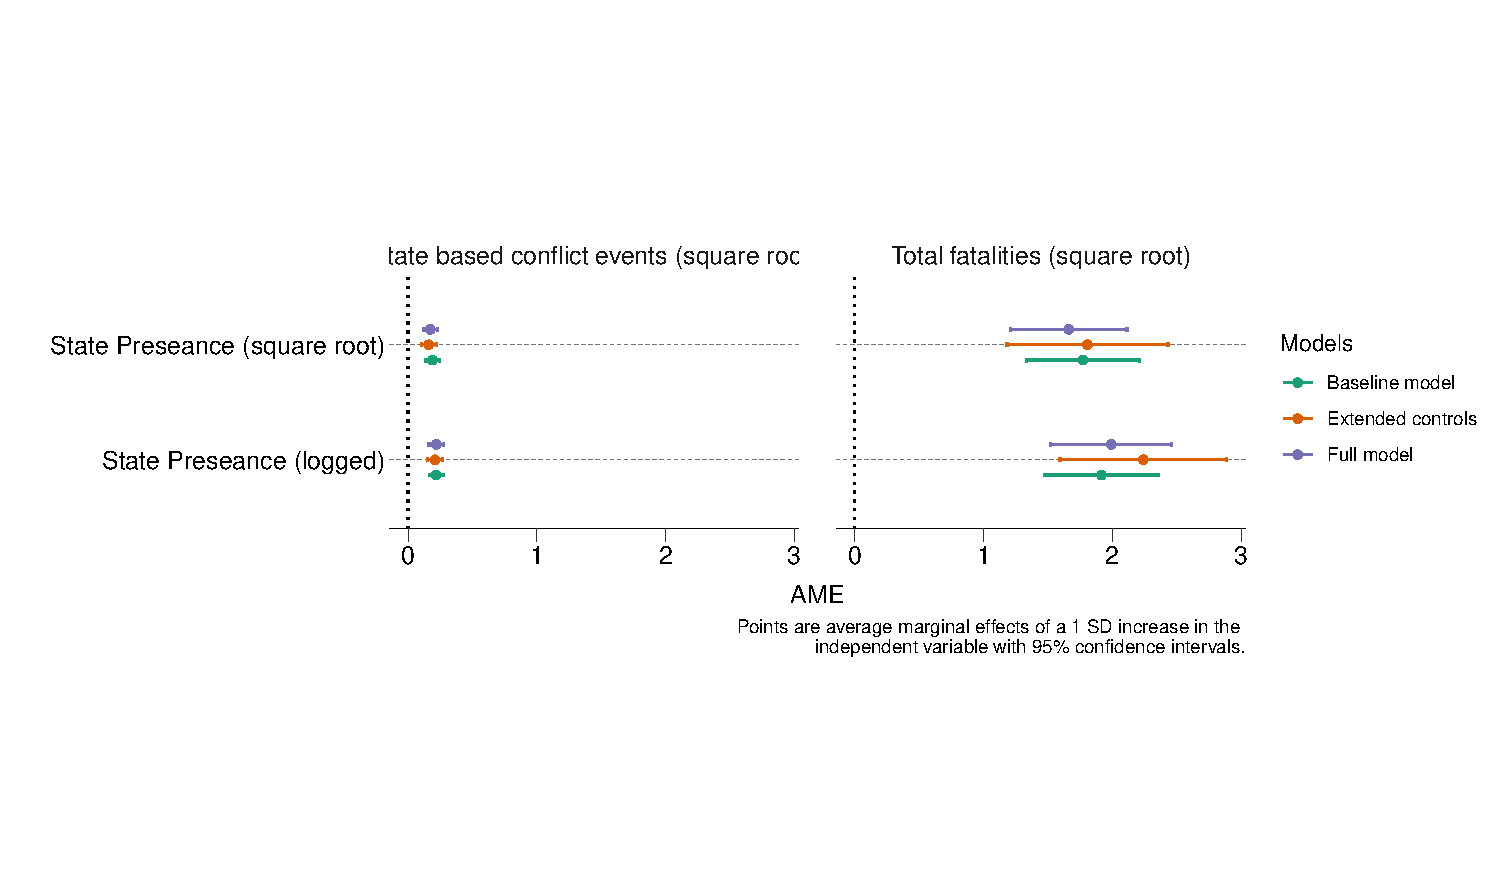
\includegraphics[width=\linewidth]{"../R/Output/conflictMargins.pdf"}
	\caption{}
	\label{margins}
\end{figure}

\section{Conclusion}

\pagebreak

\bibliographystyle{agsm}
\bibliography{../lib.bib}

\section*{Appendix}


\begin{sidewaystable}
\begin{center}
\scalebox{1}{
\begin{tabular}{l c c c c c c}
\hline
 & Baseline & Extetended Controls & Full Model & Baseline & Extetended Controls & Full Model \\
\hline
(Intercept)     & $0.50^{***}$  & $-0.23^{**}$  & $-3.02^{***}$  & $0.31^{***}$  & $-0.40^{***}$ & $-3.26^{***}$ \\
                & $(0.08)$      & $(0.09)$      & $(0.26)$       & $(0.09)$      & $(0.09)$      & $(0.26)$      \\
sqrtSpAny       & $0.11^{***}$  & $0.08^{***}$  & $0.09^{***}$   &               &               &               \\
                & $(0.01)$      & $(0.01)$      & $(0.01)$       &               &               &               \\
mountains\_mean & $1.10^{***}$  & $0.62^{***}$  & $1.03^{***}$   & $1.13^{***}$  & $0.66^{***}$  & $1.08^{***}$  \\
                & $(0.13)$      & $(0.12)$      & $(0.13)$       & $(0.13)$      & $(0.12)$      & $(0.13)$      \\
water\_gc       & $0.01^{***}$  & $0.01^{***}$  & $0.01^{***}$   & $0.01^{***}$  & $0.01^{***}$  & $0.01^{***}$  \\
                & $(0.00)$      & $(0.00)$      & $(0.00)$       & $(0.00)$      & $(0.00)$      & $(0.00)$      \\
barren\_gc      & $-0.02^{***}$ & $-0.01^{***}$ & $-0.01^{***}$  & $-0.02^{***}$ & $-0.01^{***}$ & $-0.01^{***}$ \\
                & $(0.00)$      & $(0.00)$      & $(0.00)$       & $(0.00)$      & $(0.00)$      & $(0.00)$      \\
distcoast       & $0.00^{***}$  & $0.00^{***}$  & $0.00^{***}$   & $0.00^{***}$  & $0.00^{***}$  & $0.00^{***}$  \\
                & $(0.00)$      & $(0.00)$      & $(0.00)$       & $(0.00)$      & $(0.00)$      & $(0.00)$      \\
logPopd         &               & $0.77^{***}$  & $0.83^{***}$   &               & $0.77^{***}$  & $0.83^{***}$  \\
                &               & $(0.05)$      & $(0.05)$       &               & $(0.05)$      & $(0.05)$      \\
temp\_sd        &               &               & $0.84^{***}$   &               &               & $0.81^{***}$  \\
                &               &               & $(0.10)$       &               &               & $(0.10)$      \\
temp            &               &               & $0.06^{***}$   &               &               & $0.06^{***}$  \\
                &               &               & $(0.01)$       &               &               & $(0.01)$      \\
prec\_sd        &               &               & $0.01^{\cdot}$ &               &               & $0.01^{*}$    \\
                &               &               & $(0.00)$       &               &               & $(0.00)$      \\
prec\_gpcc      &               &               & $0.00^{\cdot}$ &               &               & $0.00$        \\
                &               &               & $(0.00)$       &               &               & $(0.00)$      \\
forest\_gc      &               &               & $0.00$         &               &               & $0.00$        \\
                &               &               & $(0.00)$       &               &               & $(0.00)$      \\
logSpAny        &               &               &                & $0.25^{***}$  & $0.20^{***}$  & $0.21^{***}$  \\
                &               &               &                & $(0.02)$      & $(0.02)$      & $(0.02)$      \\
\hline
AIC             & $29551.90$    & $29272.50$    & $29042.38$     & $29530.66$    & $29250.65$    & $29019.86$    \\
BIC             & $29602.71$    & $29330.56$    & $29136.69$     & $29581.47$    & $29308.71$    & $29114.18$    \\
Log Likelihood  & $-14768.95$   & $-14628.25$   & $-14508.19$    & $-14758.33$   & $-14617.33$   & $-14496.93$   \\
Deviance        & $5709.62$     & $5757.30$     & $5778.43$      & $5713.03$     & $5759.00$     & $5778.60$     \\
Num. obs.       & $10492$       & $10482$       & $10453$        & $10492$       & $10482$       & $10453$       \\
\hline
\multicolumn{7}{l}{\scriptsize{$^{***}p<0.001$; $^{**}p<0.01$; $^{*}p<0.05$; $^{\cdot}p<0.1$}}
\end{tabular}
}
\caption{Deaths (square root)}
\label{sqrtDeaths}
\end{center}
\end{sidewaystable}


\begin{sidewaystable}
\begin{center}
\scalebox{1}{
\begin{tabular}{l c c c c c c}
\hline
 & Baseline & Extetended Controls & Full Model & Baseline & Extetended Controls & Full Model \\
\hline
(Intercept)     & $-1.07^{***}$ & $-1.65^{***}$  & $-4.43^{***}$ & $-1.25^{***}$ & $-1.79^{***}$  & $-4.58^{***}$ \\
                & $(0.07)$      & $(0.08)$       & $(0.24)$      & $(0.08)$      & $(0.09)$       & $(0.24)$      \\
sqrtSpAny       & $0.10^{***}$  & $0.06^{***}$   & $0.06^{***}$  &               &                &               \\
                & $(0.01)$      & $(0.01)$       & $(0.01)$      &               &                &               \\
mountains\_mean & $0.57^{***}$  & $0.12$         & $0.63^{***}$  & $0.59^{***}$  & $0.14$         & $0.65^{***}$  \\
                & $(0.11)$      & $(0.11)$       & $(0.12)$      & $(0.11)$      & $(0.11)$       & $(0.12)$      \\
water\_gc       & $0.01^{***}$  & $0.00^{\cdot}$ & $0.01^{**}$   & $0.01^{***}$  & $0.00^{\cdot}$ & $0.01^{**}$   \\
                & $(0.00)$      & $(0.00)$       & $(0.00)$      & $(0.00)$      & $(0.00)$       & $(0.00)$      \\
barren\_gc      & $-0.02^{***}$ & $-0.01^{***}$  & $-0.01^{***}$ & $-0.02^{***}$ & $-0.01^{***}$  & $-0.01^{***}$ \\
                & $(0.00)$      & $(0.00)$       & $(0.00)$      & $(0.00)$      & $(0.00)$       & $(0.00)$      \\
distcoast       & $0.00$        & $0.00$         & $0.00^{*}$    & $0.00$        & $0.00$         & $0.00^{*}$    \\
                & $(0.00)$      & $(0.00)$       & $(0.00)$      & $(0.00)$      & $(0.00)$       & $(0.00)$      \\
logPopd         &               & $0.68^{***}$   & $0.79^{***}$  &               & $0.67^{***}$   & $0.78^{***}$  \\
                &               & $(0.04)$       & $(0.04)$      &               & $(0.04)$       & $(0.04)$      \\
temp\_sd        &               &                & $0.93^{***}$  &               &                & $0.92^{***}$  \\
                &               &                & $(0.08)$      &               &                & $(0.08)$      \\
temp            &               &                & $0.06^{***}$  &               &                & $0.06^{***}$  \\
                &               &                & $(0.01)$      &               &                & $(0.01)$      \\
prec\_sd        &               &                & $0.01^{**}$   &               &                & $0.01^{**}$   \\
                &               &                & $(0.00)$      &               &                & $(0.00)$      \\
prec\_gpcc      &               &                & $-0.00$       &               &                & $-0.00$       \\
                &               &                & $(0.00)$      &               &                & $(0.00)$      \\
forest\_gc      &               &                & $-0.00$       &               &                & $0.00$        \\
                &               &                & $(0.00)$      &               &                & $(0.00)$      \\
logSpAny        &               &                &               & $0.23^{***}$  & $0.16^{***}$   & $0.16^{***}$  \\
                &               &                &               & $(0.02)$      & $(0.02)$       & $(0.02)$      \\
\hline
AIC             & $15439.95$    & $15148.15$     & $14813.04$    & $15407.83$    & $15123.10$     & $14790.74$    \\
BIC             & $15490.76$    & $15206.21$     & $14907.35$    & $15458.64$    & $15181.16$     & $14885.05$    \\
Log Likelihood  & $-7712.98$    & $-7566.08$     & $-7393.52$    & $-7696.92$    & $-7553.55$     & $-7382.37$    \\
Deviance        & $4776.78$     & $4835.93$      & $4907.27$     & $4793.06$     & $4843.87$      & $4911.59$     \\
Num. obs.       & $10492$       & $10482$        & $10453$       & $10492$       & $10482$        & $10453$       \\
\hline
\multicolumn{7}{l}{\scriptsize{$^{***}p<0.001$; $^{**}p<0.01$; $^{*}p<0.05$; $^{\cdot}p<0.1$}}
\end{tabular}
}
\caption{State based conflict events (square root)}
\label{sqrtState_based}
\end{center}
\end{sidewaystable}


\end{document}

